\documentclass[12pt]{report}
\usepackage{outline}
\usepackage{graphicx}
\graphicspath{ {images/} }
\usepackage{pmgraph}
\usepackage[normalem]{ulem}
\usepackage{nameref}
\usepackage{varioref}
\usepackage{hyperref}
\usepackage{cleveref}
\title{\textbf{CMPS 242 - Fall 17 \\Homework 5 - Report\\ }}
\author{Nursultan Kabylkas\\ Ramesh Jayaraman \\}
\date{\oldstylenums{11}/\oldstylenums{17}/\oldstylenums{2017}}
%--------------------Make usable space all of page
\setlength{\oddsidemargin}{0in}
\setlength{\evensidemargin}{0in}
\setlength{\topmargin}{0in}
\setlength{\headsep}{-.25in}
\setlength{\textwidth}{6.5in}
\setlength{\textheight}{8.5in}
%--------------------Indention
\setlength{\parindent}{1cm}

\begin{document}
%--------------------Title Page
\maketitle

\pagebreak
%--------------------Page 2-------------------
 
\section*{1. Introduction} 

%--------This section will contain a brief intro to the project and will list all other things in this pdf.

The objective of this project it to classify tweets, tweeted by Hillary Clinton and Donald Trump. This was achieved by implementing a LSTM Recurrent Neural Net, using tensor flow, training it with the data provided, and tested using the test data set provided. The results from the test set were submitted to Kaggle, to rank different implementations by their accuracy.\\

	This report is structured to provide an introduction to the work done, followed by the details of the implementation, and then the results that were obtained. 	

\section*{2. Implementation}

%----------This part will give a a short intro to implementation and will flow into pre-processing subsection.

In this section, we explain all aspects of our implementation, starting with the characteristics of the input data set, how we perform pre-processing, then tokenize the data. We then give details about the implementation of our Recurrent Neural Net, and how we train it.

\subsection*{2.1 Data set characteristics}
%-----give details about the data set, lead to preprocessing

The input data set has the format as shown in Figure \ref{input}. The input file was formatted as a comma-separated values (".csv") file, where the different fields are separated by commas. 

\begin{figure}[h]
\centering
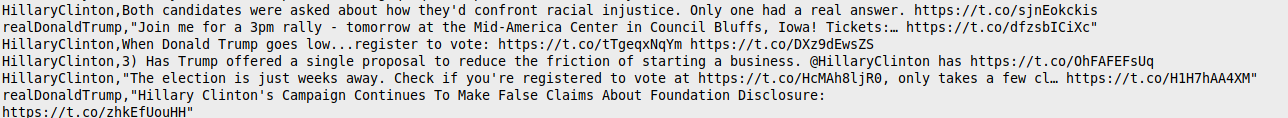
\includegraphics[scale=.36]{inputs.png}
\caption{This image shows the format of the input file.} \label{input}
\end{figure}

The first field is the Twitter handle of the candidate, which serves as the label for the tweet, HillaryClinton (Hillary Clinton), realDonaldTrump (Donald Trump). The second field contains the tweet. There were a total of 4743 tweets in the input data set.

The test data set was given in the same format, ie. a .csv file, containing a total of 1701 tweets, but had the handle replaced with "none". 

	As we could not validate our predictions due to the absence of labels in the test data set, we formatted our results as a .csv file, with three fields, the first of which was the tweet id,
\subsection*{2.2 Preprocessing }

Talk about preprocessing that we did and flow into token stuff.

\subsection*{2.3 Tokenizing}

Talk about how we tokenized. lead into rnn section

\subsection*{2.4 rnn implementation}

talk about rnn implementation and tensor flow. Lead into training

\subsection*{2.5 training}
talk about training, and then lead into testing and results.

\section*{3.Results}

Give intro to what we ran, config etc.

\subsection*{3.1 rnn results}

give results from rnn

\subsection*{3.2 Compare with logistic regression}

Compare it with logistic.

\section*{4. Conclusion}
Conclude work.

\end{document}